\documentclass{article}
\usepackage{graphicx}
\graphicspath{ {images/} }
\begin{document}
\section*{Personas}
\subsection*{Sarah Garrell (20)}
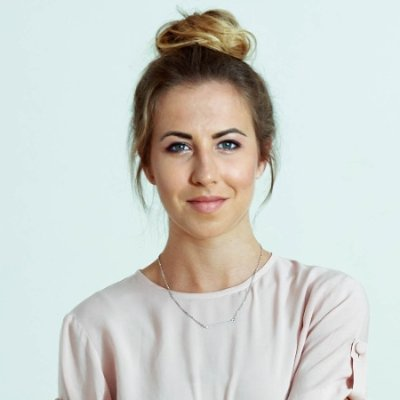
\includegraphics[scale=0.5]{sarah.png}\\
\textbf{Job Title: }1st year HR student\\
\textbf{Education:} High School + CEGEP\\
\textbf{Experience:}
\begin{itemize}
\itemsep0em 
\item Starbucks Barista
\item Summer camp counselor
\item Plays piccolo
\end{itemize}
\textbf{Goals:}
\begin{itemize}
\itemsep0em 
\item Get her degree and work in recruiting
\item Pass accounting and finance
\end{itemize}

\subsection*{Goals and Tasks user accomplishes}
Mostly she is worried about her finance class so anything that would help her with that would be appreciated.
\subsection*{Problem calculator solves}
She needs a calculator to calculate the equations for finance class. Her school does not allow her a programmable calculator so she will need to memorize the equations. She would definitely appreciate a it if she could enter the equation from left to right just like she memorized them.
\pagebreak

\subsection*{Interview Q\&A}
\textbf{What do you use a calculator for?}
\begin{itemize}
\itemsep0em 
\item Almost exclusively for her accounting and finance classes
\item Most of her usage of the calculator is for simple lightweight math used in accounting and finance.
\item She does not use it extensively, mostly for exams and homework.
\end{itemize}

\textbf{What would you like your calculator to do? Or what is the ideal calculator for you?}
\begin{itemize}
\itemsep0em 
\item She likes her calculator to be simple
\item Prefers a calculator that has its function symbols identical to the ones in the books
\item She would like her calculator to display the answers in a human readable form (5x7 Matrix numeric representation), and not the digital form (7-segment numeric representation)
\item In the future she would like to see a calculator network system, similar to that of the iclicker, where the professor would give you a password, which after inputting it into the calculator, downloads a custom function from the professor's base station, or unlocks/locks some of the pre programmed functions in the calculator.
\end{itemize}

\textbf{What kinds of calculators have you used? (physical, apps, online, etc.). Hardware or Software?}
\begin{itemize}
\itemsep0em 
\item Uses both a physical calculator as well as a calculator app on her phone.
\item Mainly uses the calculator application because it’s always available.
\item Prefers the physical calculator since she enjoys the tactile feel of the buttons and because phones are not allowed during exam time.
\end{itemize}

\textbf{What functions do you use most often? Which ones do you use the least?}
\begin{itemize}
\itemsep0em 
\item Most of the time she uses functions such as: addition, subtraction, delete (backspace) , $10^x$, Ans function for retrieving the previous answer , exponential and square root.
\item Rarely, if ever, uses logarithms or any of the trigonometric functions.
\end{itemize}

\textbf{What features did you like most about your calculator. What do you not like about your calculator?}
\begin{itemize}
\itemsep0em 
\item She feels indifferent about what she likes in her calculator. All she cares about is that the calculator gives the right answer.
\item The only thing she does not like about her calculator is that it displays numbers in a digital format (7 segment numeric representation)
\end{itemize}

\textbf{Are the aesthetics of your calculator important? What matters most (shape, color,  personalized themes, etc.)?}
\begin{itemize}
\itemsep0em 
\item Most of the physical aesthetics are of little importance to her. What matters the most is that the calculator gives an answer.
\item She claims that the physical aesthetics would be merely a perk and would not pay extra for them.
\end{itemize}

\textbf{If you’re using a keyboard, how would you map the keys to functions, numbers, etc. ergonomics?}
\begin{itemize}
\itemsep0em 
\item She would like her calculator to have some shortcuts to common functions such as percentage 
\item Prefers the shortcuts to have their own dedicated buttons on the calculator instead of having to press multiple buttons at once.
\end{itemize}

\textbf{Thoughts on making a calculator that has customizable capabilities? }
\begin{itemize}
\itemsep0em 
\item She would like to have the ability to program functions into the calculator, but only if academic establishments would allow it. 
\end{itemize}
\pagebreak

\subsection*{Kevin Donnavan (23)}
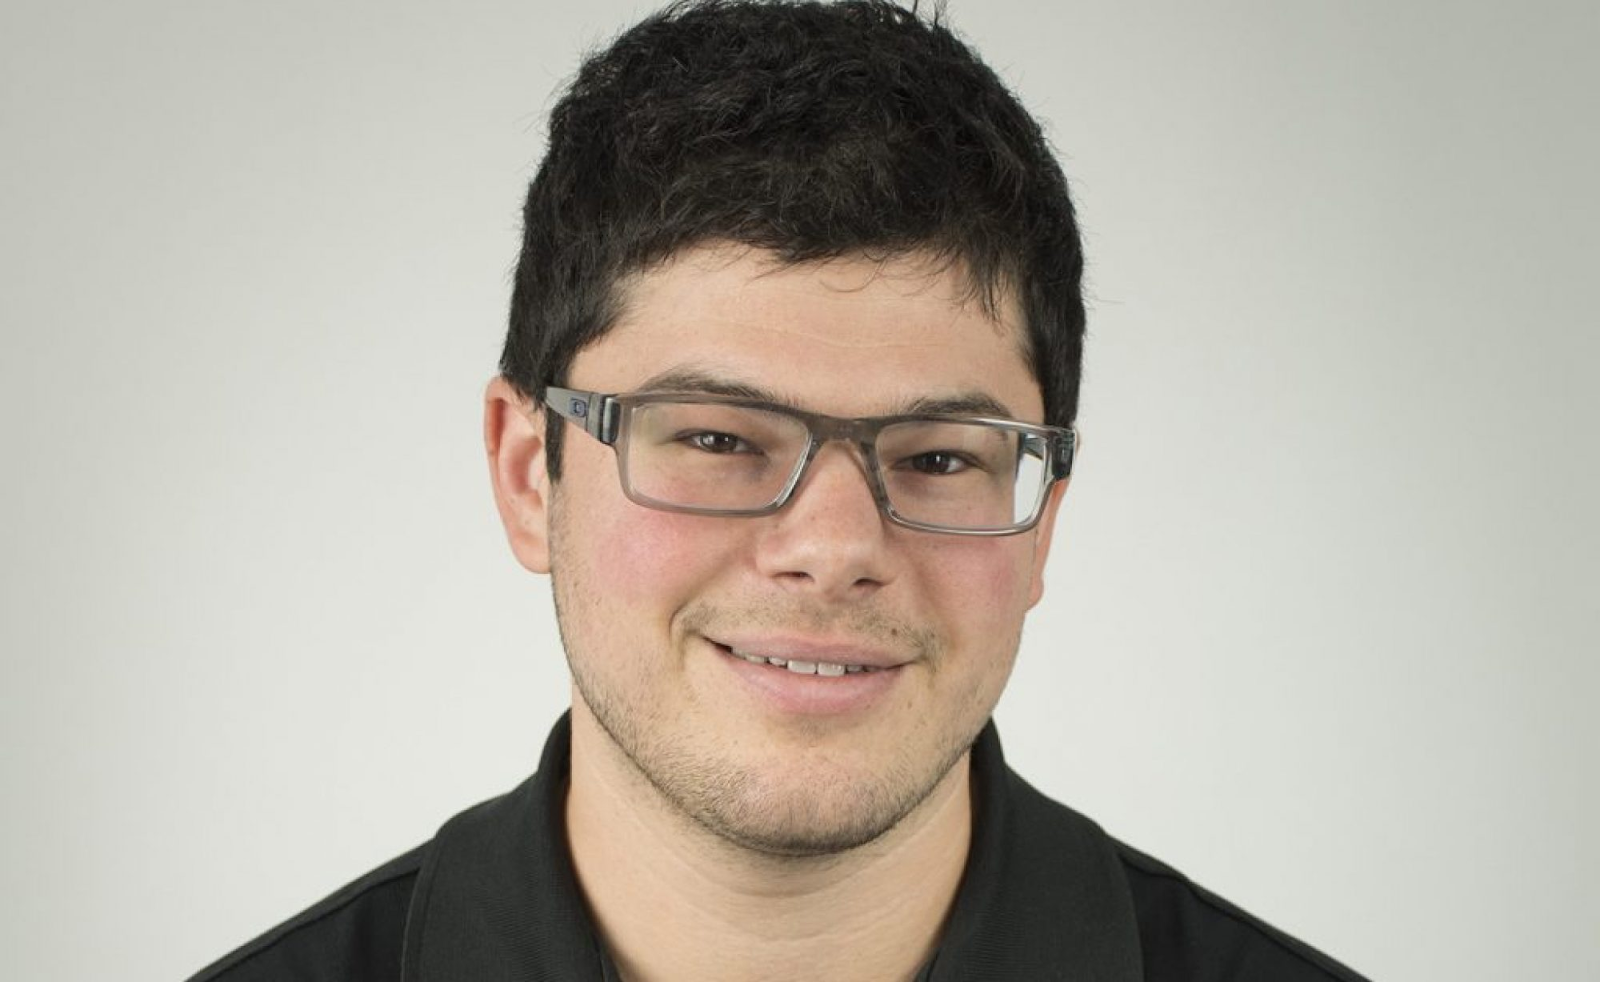
\includegraphics[scale=0.15]{kevin.png}\\
\textbf{Job Title: }Engineering Student\\
\textbf{Education:} 3rd Year Mechanical Engineering\\
\textbf{Experience:}
\begin{itemize}
\itemsep0em 
\item 3rd Year Mechanical Engineering
\item Summer internship as a junior structural engineer
\item Army reserves - Infantry
\end{itemize}

\textbf{Skills:}
\begin{itemize}
\itemsep0em 
\item Problem Solving, Mathematics
\item Programming in Java, C\#, and C++
\end{itemize}

\textbf{Goals:}
\begin{itemize}
\itemsep0em 
\item Obtain a good GPA and find a job in his field.
\end{itemize}

\subsection*{Goals and Tasks user accomplishes}
Kevin says he just wants to get through his classes and get a decent GPA. Like everyone, his hardest classes mostly have to do with math (although he feels he is better than average). Kevin will be happy with anything that can make his math calculations easier. 
\subsection*{Problem calculator solves}
The calculator helps Kevin get fast answers to difficult math problems he sees in class. Without a calculator, he is not sure how he would calculate the various functions that he sees on a daily basis. The calculator has to be precise enough so he can get the right answer to complex solutions of differential equations but he is not willing to wait - calculation must be near-instantaneous.
\pagebreak

\subsection*{Interview Q\&A}
\textbf{What do you use a calculator for?}
\begin{itemize}
\itemsep0em 
\item University studies
\item Mostly finds himself using it for mathematical purposes. 
\end{itemize}

\textbf{What would you like your calculator to do? Or what is the ideal calculator for you?}
\begin{itemize}
\itemsep0em 
\item His  ideal calculator would not be missing essential functions like plus, minus, multiplication, exponents, and the basics. Other common functions he mentioned from University, include logs, derivatives, e, integrals, roots, square roots, and more. He believes it’s a must to have the ANS (answer button), and calculation history included too. 
\item The calculator should be lightweight and portable. 
\item In the future he would like to see more calculators that provide more support for polar coordinates. Lastly he would like to have access to shorter readable manuals or video content to quickly go over all of the calculator’s features and how to implement them.
\item Believes It would be great to have the answer button, calculation history, polar capability and a shorter readable manual! 
\end{itemize}

\textbf{What kinds of calculators have you used? (physical, apps, online, etc.). Hardware or Software?}
\begin{itemize}
\itemsep0em 
\item Both softwares and physical.
\item Prefers physical calculator more than software-based because he has become used to it since his High School years. 
\item He doesn’t mind using software calculators as long as it has useful shortcuts. He defined a simple software calculator as something that can open and run quickly on a computer or any other device. 
\item Kevin also mentioned he uses software calculators mostly for basic problems but not derivations and more advanced operations because it becomes too tedious to work with. He would much rather use the physical one. 
\end{itemize}

\textbf{What functions do you use most often? Which ones do you use the least?}
\begin{itemize}
\itemsep0em 
\item Addition, subtraction, multiplication, division, exponents, roots, converting to fractions, sin, cos, tan, exponents, logs, and mod.
\end{itemize}

\textbf{What features did you like most about your calculator. What do you not like about your calculator?}
\begin{itemize}
\itemsep0em 
\item He liked Hexadecimal conversion, octa, binary conversions, derivations, and integration functions because they’re relevant to his engineering courses. .
\item Kevin doesn’t like using the mouse pointer on his computer to input the values and functions on his software-based calculator. He would much rather use the computer keyboard. He mentioned the clicking option should be removed completely to encourage others to use the keyboard. 
\end{itemize}

\textbf{Are the aesthetics of your calculator important? What matters most (shape, color,  personalized themes, etc.)?}
\begin{itemize}
\itemsep0em 
\item Easy to fit in your palm, portable, not too colourful (greyish, black). It should also be key mappable if it is a software-based calculator.
\end{itemize}

\textbf{If you’re using a keyboard, how would you map the keys to functions, numbers, etc. ergonomics?}
\begin{itemize}
\itemsep0em 
\item He would use the numbered keypad for inputting numbers 
\item Any symbols that are already commonly found (+,-,\^,etc.) on both computers and physical calculators should be included.
\item Assign important features and functions to large buttons, like the space bar or return key.
\item Include a shortcut to quit
\item Use the first letter of functions to input them into calculator. Ex: C for cos, S for sin, T for Tan, etc.
\end{itemize}

\textbf{Thoughts on making a calculator that has customizable capabilities? }
\begin{itemize}
\itemsep0em 
\item Doesn’t think it is necessary. He usually uses google to help solve complex problems and inputs the simple calculations on the calculator to double check his work and find the final answer. 
\item He believes it would be great to include physical skins to personalize the calculator but it is not a must.
\item In the future he would like to make it customizable by being able to download packages for calculator functions that can easily be added or removed to the device.
\end{itemize}
\pagebreak

\subsection*{Tarek Ghamzi (23)}

\includegraphics[scale=0.25]{tarek.jpg}\\
\textbf{Job Title: }3rd year Electrical engineering student\\
\textbf{Education:} High School + CEGEP, currently in Electrical Engineering\\
\textbf{Experience:}
\begin{itemize}
\itemsep0em 
\item Subway
\item Pharmacist assistant
\end{itemize}

\textbf{Skills:}
\begin{itemize}
\itemsep0em 
\item Problem Solving, Mathematics
\item Programming in C++ , and arduino 
\end{itemize}

\textbf{Goals:}
\begin{itemize}
\itemsep0em 
\item Finish his degree with a good GPA
\item Find a job in his field
\end{itemize}

\subsection*{Goals and Tasks user accomplishes}
Tarek claims that his main priority in life at the moment is to get his degree in Electrical Engineering. He claims that his field is heavily based on math, which he struggles with.
He aims to graduate with a higher than average GPA to gain an edge over others in his highly competitive field.

\subsection*{Problem calculator solves}
His calculator helps him in computing the high level mathematical functions that would take hours to solve by himself. It also helps him double check his answers for simple calculations.
Tarek claims that his calculator is with him at all times. Its accuracy, speed and comfort are of highest value to him.

\pagebreak

\end{document}